\section{Analysis}
Indentation at the top of the chip (\autoref{fig:sub4}) determines where the top is and helps to indicate which pin is which.  Basic pin setup is: $V_{in}(+)$ is the analog input, and $DO$ is the serial output. $V_{ref}$ and   $Vin(-)$ are used calibrate chip by applying certain voltage. $V_{dd}$ $(V_{cc})$ and $GND$ are used for supplying power to the chip. $CS$ is for active low chip set, and $CLK$ is for clock. So, to take measurements using chip, the $CS$ pin must receive a signal from the Raspberry Pi that starts high and goes low. This signal should stay low until you end your program. $CLK$ input must receive a single clock pulse to state that the conversation should start at the next clock pulse. For this chip, a clock pulse starts low, sets high, and goes low again, 8 more clock pulses are required to complete the conversation. Each time a clock pulse is received by $CLK$, another of the serial bits is sent by the $DO$ output. See \autoref{fig:finalcircuit} for final setup.
\begin{figure}[h]
\centering
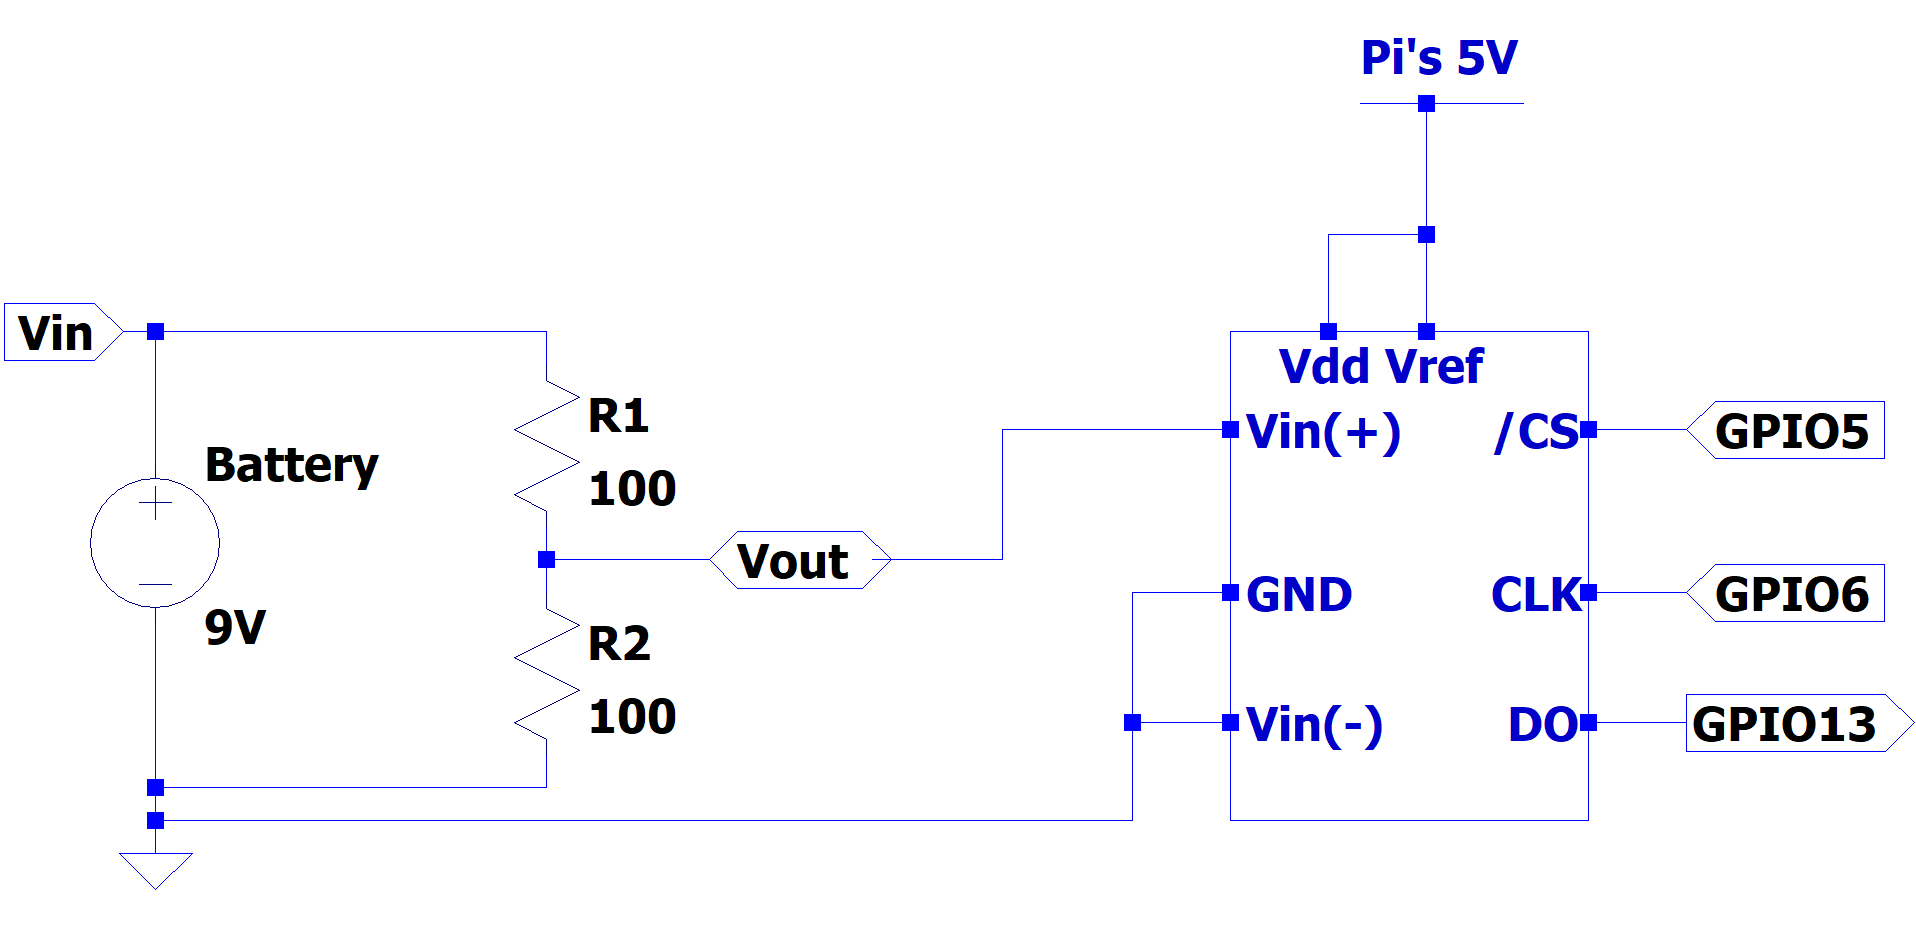
\includegraphics[width=0.9\textwidth]{finalcircuit.png}
\caption{Final Circuit Build}
\label{fig:finalcircuit}
\end{figure}\newline
According to ADC0831 datasheet\citep{adcdatasheet}, the chip is limited to measure only up to about 5V, so 9V straight into the chip might cause some problems. That is why voltage divider is utilized: letting both resistors $R_1$ and $R_2$ to be equal to each other \autoref{eq:voltdiv} will be $V_{out} = V_{in}/2$, where $V_{in}$ is the battery voltage. Assuming battery has a steady current draw of 45 mA(5 pins in use)\citep{current}, applying \autoref{eq:current}, we get $R_1 = R_2 = R=104.2\Omega$. The voltmeter reading was $V_{in} = V_{battery} = 9.257V$, resulting $V_{out} = 4.606V$. To be more precise with the factor of 2, $V_{in}$ and $V_{out}$ were measured with voltmeter to be $V_{in} = V_{battery} = 9.257V$, resulting $V_{out} = 4.606V$, the factor of about 2.01 was obtained. Basically, multiplying voltage reading from the chip by 2.01, allows the battery voltage calculation to be more precise. \newline
Raspberry Pi was left to record voltage value every minute. See \autoref{fig:datavis} for graph representation of data.\citep{project} 
Linear regression was applied to period where the discharge is steady letting us to calculate battery capacity. Regression is on $t \in[2.55,11.32]$, giving us the capacity:
\begin{equation}
    {Capacity} = {I}*{\Delta t} = 45 * 8.77 = 394.65 \ mA*h
    \label{eq:capacity}
\end{equation}{}

\begin{figure}[t]
\centering
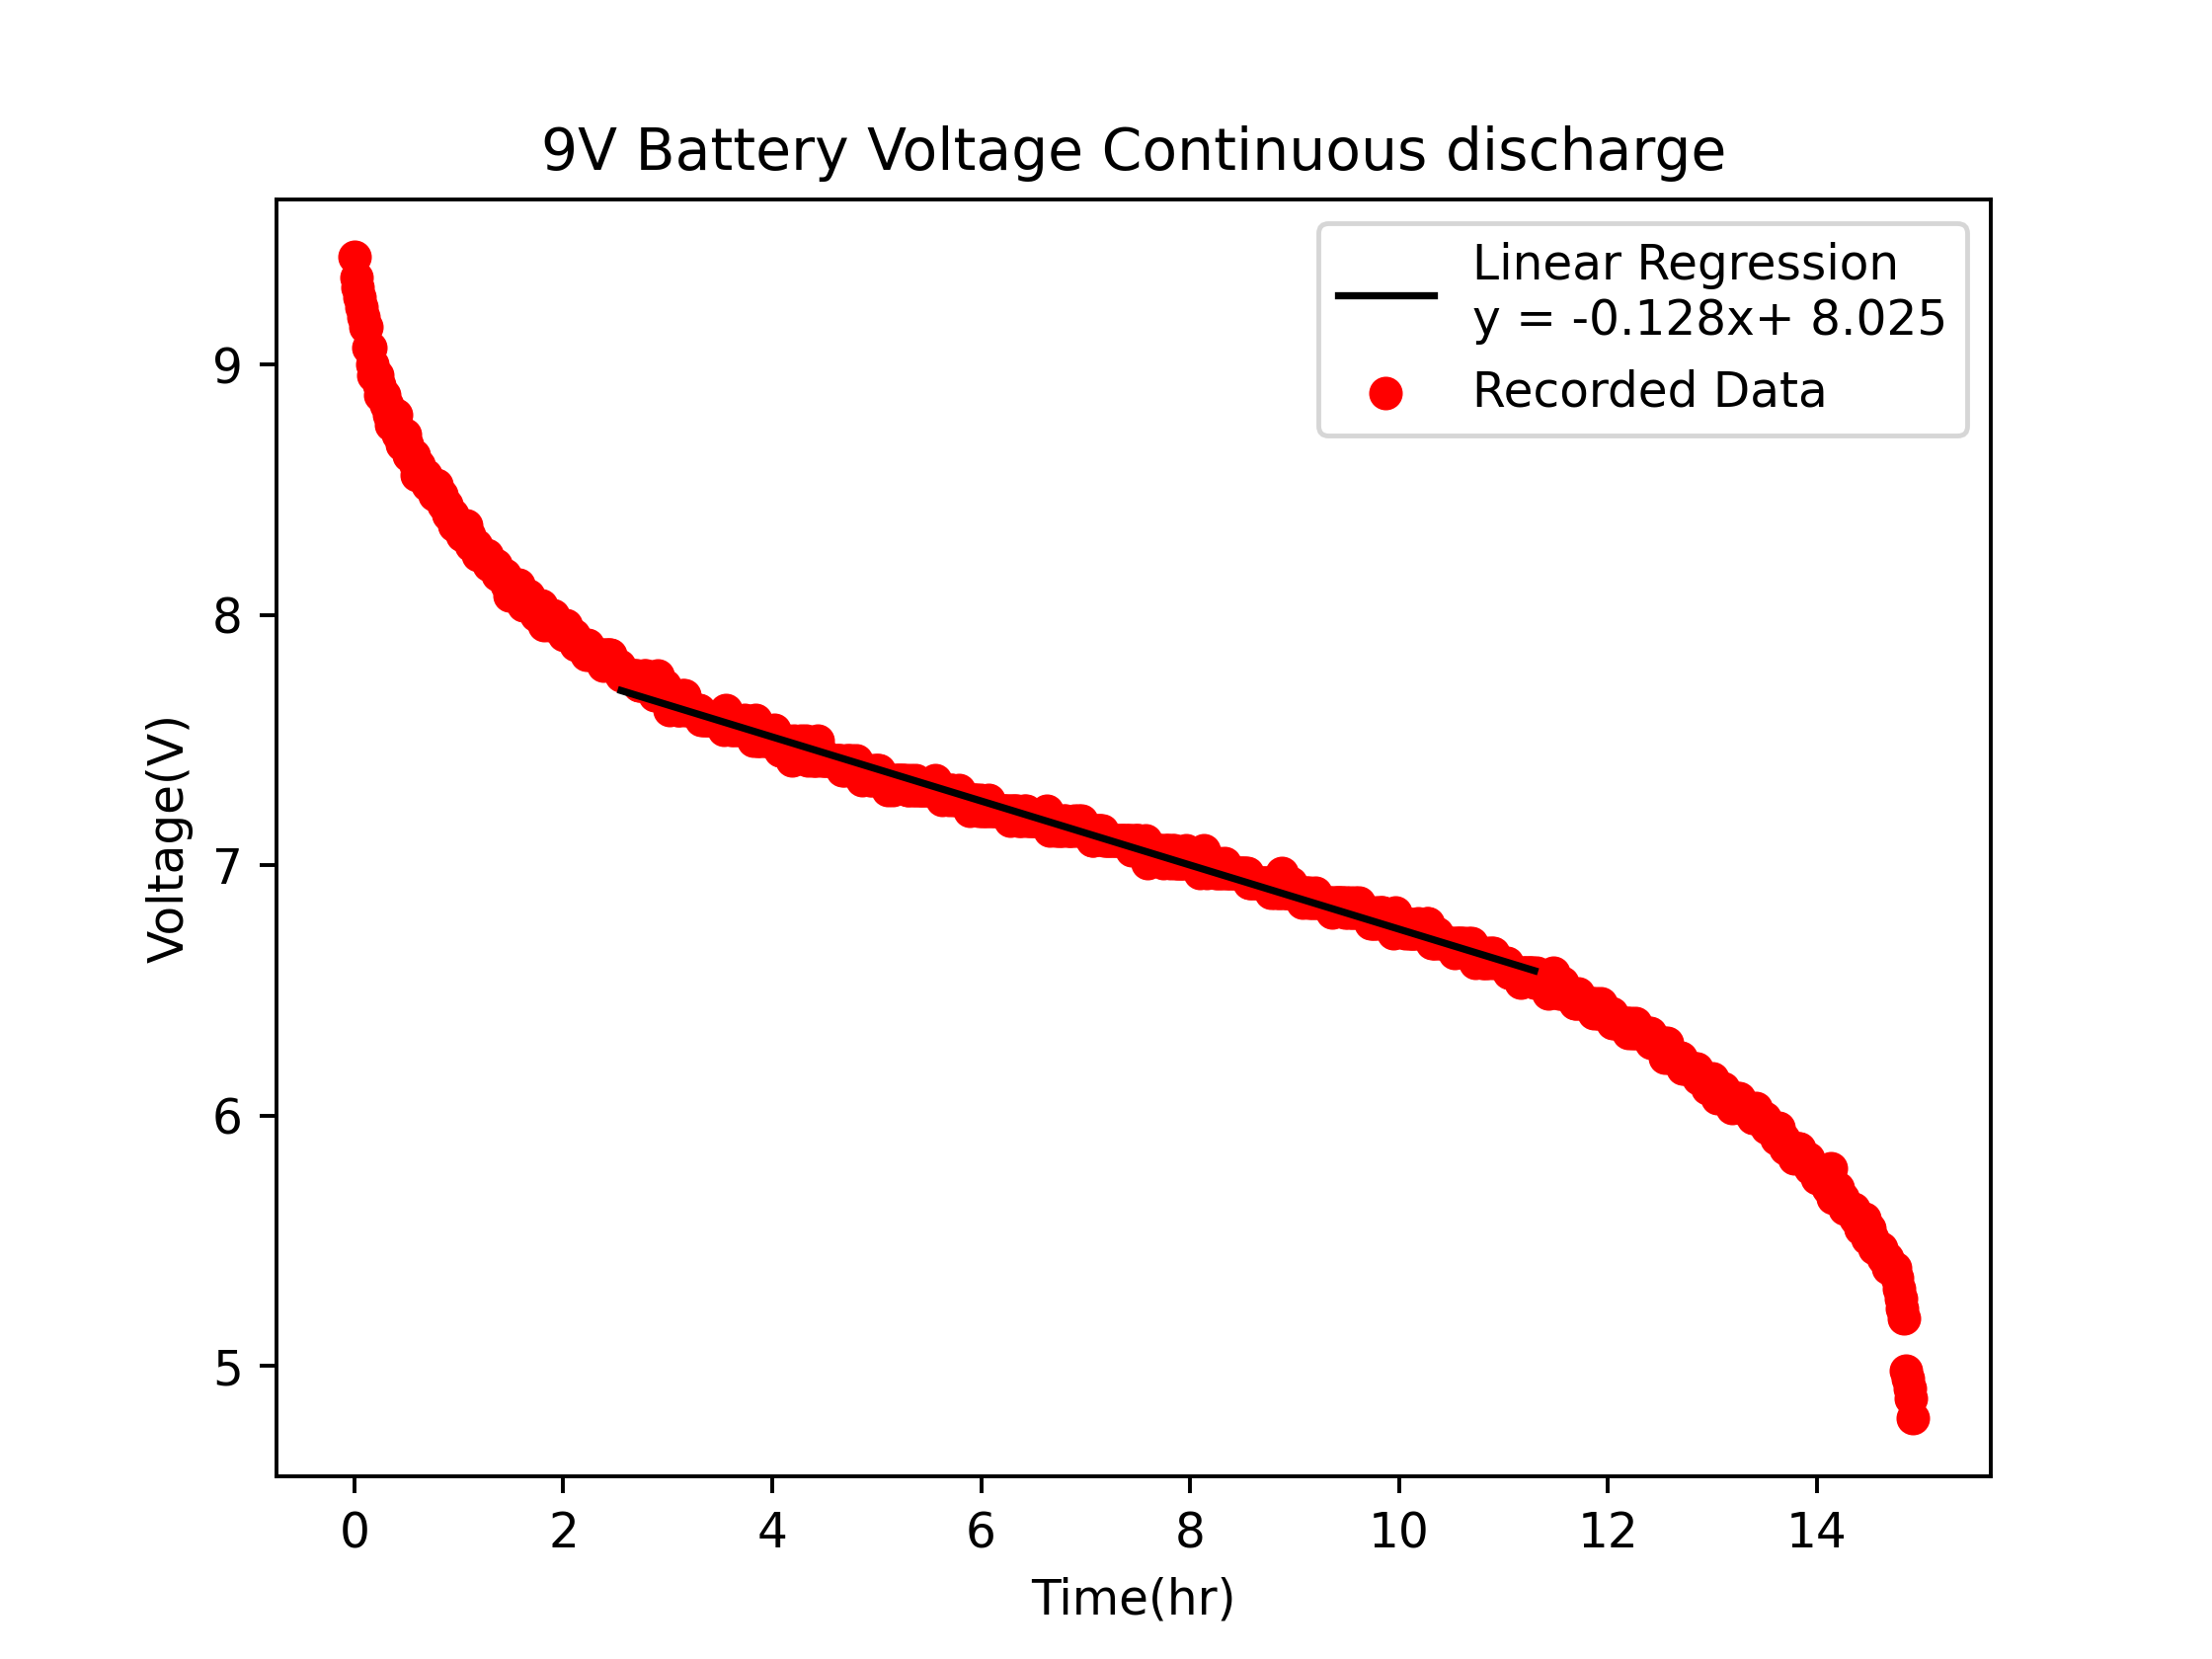
\includegraphics[width=0.8\textwidth]{ex1test.png}
\caption{Data Visualization}
\label{fig:datavis}
\end{figure}